%%%%%%%%%%%%%%%%%%%%%%%%%%%%%%%%%%%%%%%%%%%%%%%%%%%%%%%%%%%%%%%%%%%%%%%%%%%%%%%%%%%%%%%%%%
% Ceci est le fichier principal du template template à utiliser pour les rapports du     %
% projet 1 (Construction de Programme) d'INFO0947.                                       %
%                                                                                        %
% Vous devez décommenter et compléter les commandes introduites plus bas (intitule, ...) %
% avant de pouvoir compiler le fichier LaTeX.  Pensez à configurer votre Makefile en     %
% conséquence.                                                                           %
%                                                                                        %
% Le contenu et la structure du rapport sont imposés.  Vous devez compléter les          %
% différents fichiers .tex inclus dans ce fichier avec votre production.                 %
%%%%%%%%%%%%%%%%%%%%%%%%%%%%%%%%%%%%%%%%%%%%%%%%%%%%%%%%%%%%%%%%%%%%%%%%%%%%%%%%%%%%%%%%%%

% !TEX root = ./main.tex
% !TEX engine = latexmk -pdf
% !TEX buildOnSave = true
\documentclass[a4paper, 11pt, oneside]{article}

\usepackage[utf8]{inputenc}
\usepackage[T1]{fontenc}
\usepackage[french]{babel}
\usepackage{array}
\usepackage{shortvrb}
\usepackage{listings}
\usepackage[fleqn]{amsmath}
\usepackage{amsfonts}
\usepackage{fullpage}
\usepackage{enumerate}
\usepackage{graphicx}             % import, scale, and rotate graphics
\usepackage{subfigure}            % group figures
\usepackage{alltt}
\usepackage{url}
\usepackage{indentfirst}
\usepackage{eurosym}
\usepackage{listings}
\usepackage{color}
\usepackage[table,xcdraw,dvipsnames]{xcolor}

% Change le nom par défaut des listing
\renewcommand{\lstlistingname}{Extrait de Code}


\definecolor{mygray}{rgb}{0.5,0.5,0.5}
\newcommand{\coms}[1]{\textcolor{MidnightBlue}{#1}}

\lstset{
    language=C, % Utilisation du langage C
    commentstyle={\color{MidnightBlue}}, % Couleur des commentaires
    frame=single, % Entoure le code d'un joli cadre
    rulecolor=\color{black}, % Couleur de la ligne qui forme le cadre
    stringstyle=\color{RawSienna}, % Couleur des chaines de caractères
    numbers=left, % Ajoute une numérotation des lignes à gauche
    numbersep=5pt, % Distance entre les numérots de lignes et le code
    numberstyle=\tiny\color{mygray}, % Couleur des numéros de lignes
    basicstyle=\tt\footnotesize,
    tabsize=3, % Largeur des tabulations par défaut
    keywordstyle=\tt\bf\footnotesize\color{Sepia}, % Style des mots-clés
    extendedchars=true,
    captionpos=b, % sets the caption-position to bottom
    texcl=true, % Commentaires sur une ligne interprétés en Latex
    showstringspaces=false, % Ne montre pas les espace dans les chaines de caractères
    escapeinside={(>}{<)}, % Permet de mettre du latex entre des <( et )>.
    inputencoding=utf8,
    literate=
  {á}{{\'a}}1 {é}{{\'e}}1 {í}{{\'i}}1 {ó}{{\'o}}1 {ú}{{\'u}}1
  {Á}{{\'A}}1 {É}{{\'E}}1 {Í}{{\'I}}1 {Ó}{{\'O}}1 {Ú}{{\'U}}1
  {à}{{\`a}}1 {è}{{\`e}}1 {ì}{{\`i}}1 {ò}{{\`o}}1 {ù}{{\`u}}1
  {À}{{\`A}}1 {È}{{\`E}}1 {Ì}{{\`I}}1 {Ò}{{\`O}}1 {Ù}{{\`U}}1
  {ä}{{\"a}}1 {ë}{{\"e}}1 {ï}{{\"i}}1 {ö}{{\"o}}1 {ü}{{\"u}}1
  {Ä}{{\"A}}1 {Ë}{{\"E}}1 {Ï}{{\"I}}1 {Ö}{{\"O}}1 {Ü}{{\"U}}1
  {â}{{\^a}}1 {ê}{{\^e}}1 {î}{{\^i}}1 {ô}{{\^o}}1 {û}{{\^u}}1
  {Â}{{\^A}}1 {Ê}{{\^E}}1 {Î}{{\^I}}1 {Ô}{{\^O}}1 {Û}{{\^U}}1
  {œ}{{\oe}}1 {Œ}{{\OE}}1 {æ}{{\ae}}1 {Æ}{{\AE}}1 {ß}{{\ss}}1
  {ű}{{\H{u}}}1 {Ű}{{\H{U}}}1 {ő}{{\H{o}}}1 {Ő}{{\H{O}}}1
  {ç}{{\c c}}1 {Ç}{{\c C}}1 {ø}{{\o}}1 {å}{{\r a}}1 {Å}{{\r A}}1
  {€}{{\euro}}1 {£}{{\pounds}}1 {«}{{\guillemotleft}}1
  {»}{{\guillemotright}}1 {ñ}{{\~n}}1 {Ñ}{{\~N}}1 {¿}{{?`}}1
}
\newcommand{\tablemat}{~}

%%%%%%%%%%%%%%%%% TITRE %%%%%%%%%%%%%%%%
% Complétez et décommentez les définitions de macros suivantes :
\newcommand{\intitule}{Prefixe and Suffixe}
\newcommand{\GrNbr}{33}
\newcommand{\PrenomUN}{Aleksandr}
\newcommand{\NomUN}{Pavlov}
\newcommand{\PrenomDEUX}{}
\newcommand{\NomDEUX}{}

\renewcommand{\tablemat}{\tableofcontents}

%%%%%%%% ZONE PROTÉGÉE : MODIFIEZ UNE DES DIX PROCHAINES %%%%%%%%
%%%%%%%%            LIGNES POUR PERDRE 2 PTS.            %%%%%%%%
\title{INFO0947: \intitule}
\author{Groupe \GrNbr : \PrenomUN~\textsc{\NomUN}, \PrenomDEUX~\textsc{\NomDEUX}}
\date{}
\begin{document}

\maketitle
\newpage
\tablemat
\newpage

%%%%%%%%%%%%%%%% RAPPORT %%%%%%%%%%%%%%%

% Inclusion des différentes sections

% !TEX root = ./main.tex
%%%%%%%%%%%%%%%%%%%%%%%%%%%%%%%%%%%%%%%%%%%%%%%%%%%%%%%%%%%%%%%%%%%%%%%%%%%%%%%%%%%%%%%%%%
% Rédigez ici l'introduction de votre rapport.                                           %
%%%%%%%%%%%%%%%%%%%%%%%%%%%%%%%%%%%%%%%%%%%%%%%%%%%%%%%%%%%%%%%%%%%%%%%%%%%%%%%%%%%%%%%%%%
\section{Introduction}\label{introduction}
%%%%%%%%%%%%%%%%%%%%%%%

Dans le cadre du cours INFO-0947
nous avons du résoudre un problème donné et en créer un algorithm en C capable de:
trouver la longueur du plus grand sous-tableau qui soit a la fois le préfixe et le suffixe d'un tableau donné.
Ce problème sera complétement documenter en LaTex.
Pour ce fair, nous devons prendre compte de plusieurs contraintes:
ne pouvions pas utiliser de tableau intermédiaire
et nous avions l'obligation d'utiliser uniquement des boucles de type while.


% !TEX root = ./main.tex
%%%%%%%%%%%%%%%%%%%%%%%%%%%%%%%%%%%%%%%%%%%%%%%%%%%%%%%%%%%%%%%%%%%%%%%%%%%%%%%%%%%%%%%%%%
% Dans cette section, introduisez toutes les notations mathématiques que vous jugez      %
% utiles à la réalisation du projet.                                                     %
%%%%%%%%%%%%%%%%%%%%%%%%%%%%%%%%%%%%%%%%%%%%%%%%%%%%%%%%%%%%%%%%%%%%%%%%%%%%%%%%%%%%%%%%%%
\section{Formalisation du Problème}\label{formalisation}
%%%%%%%%%%%%%%%%%%%%%%%%%%%%%%%%%%%


\textbf{Notations clés}:\\
    $ T[0 \dots k-1] $ — préfixe de la longueur $k$ du tableau $T$\\
    $ T[N-k \dots N-1] $ — suffixe de la longueur $k$ du tableau $T$\\
\\
\textbf{Prédicat}:\\
$ \operatorname{pref\_equals\_suff}(T, N, k) \equiv (0 < k < N) \land \forall i \in [0 \dots k - 1], T[i] = T[N - k + i]$\\
\\
\textbf{Fonction}:\\
$ \operatorname{prefixe\_suffixe}(T, N) \equiv \max\{k \mid k \in [0 \dots N - 1], \operatorname{pref\_equals\_suff}(T, N, k)\} $ \\


% !TEX root = ./main.tex
%%%%%%%%%%%%%%%%%%%%%%%%%%%%%%%%%%%%%%%%%%%%%%%%%%%%%%%%%%%%%%%%%%%%%%%%%%%%%%%%%%%%%%%%%%
% Dans ce fichier, vous devez définir (Input/Output/O.U.) proprement et clairement le    %
% problème.
%
% Il est aussi demandé de réaliser une analyse complète (i.e., découpe en SPs)           %
%%%%%%%%%%%%%%%%%%%%%%%%%%%%%%%%%%%%%%%%%%%%%%%%%%%%%%%%%%%%%%%%%%%%%%%%%%%%%%%%%%%%%%%%%%

\section{Définition et Analyse du Problème}\label{analyse}
%%%%%%%%%%%%%%%%%%%%%%%%%%%%%%%%%%%%%%%%%%%%


\subsection{Input/Output}

\begin{itemize}
\item \textbf{Input}:
    Un tableau d'entiers $T$ de taille $N$: \\
    $ T = (T[0], T[1] \dots T[N - 1]) $ \\
    $ \land $ \\
    $ N \geq 0 $

\item \textbf{Output}:
    Un entier $k$ représentant la longueur maximale des sous-tableaux (préfixe et suffixe)
    du tableau $T$. \\
    $k < N \land \operatorname{pref\_equals\_suff}(T, N, k)$ \\
    \\
    Si de tels sous-tableaux n'existent pas, renvoyez 0.
\end{itemize}


\subsection{Découpe en sous-problèmes}

\begin{itemize}
\item \textbf{SP 1}: Énumération des longueurs possibles pour les préfixes et suffixes \\
    Nous parcourons toutes les longueurs possibles $k$ (pour les préfixes et suffixes)
    du tableau $T$ dans l'ordre décroissant de $N-1$ jusqu’à $1$.
    Pour chaque longueur $k$, nous vérifions la correspondance en utilisant la méthode de comparaison (SP 2).
    Dès que nous trouvons une longueur $k$ pour laquelle le préfixe et le suffixe correspondent,
    nous la retournons. \\
    Si aucune longueur ne convient, nous retournons 0.

\item \textbf{SP 2}: Vérification de l’égalité entre préfixe et suffixe \\
    Pour une longueur $k$ donnée,
    nous vérifions si le préfixe et le suffixe de $T$ sont identiques.
    Cette comparaison s’effectue élément par élément.

\end{itemize}


% !TEX root = ./main.tex
%%%%%%%%%%%%%%%%%%%%%%%%%%%%%%%%%%%%%%%%%%%%%%%%%%%%%%%%%%%%%%%%%%%%%%%%%%%%%%%%%%%%%%%%%%
% Dans cette section, spécifiez formellement chacun des sous-problèmes.                  %
%%%%%%%%%%%%%%%%%%%%%%%%%%%%%%%%%%%%%%%%%%%%%%%%%%%%%%%%%%%%%%%%%%%%%%%%%%%%%%%%%%%%%%%%%%
\section{Specifications}\label{specifications}
%%%%%%%%%%%%%%%%%%%%%%%%



\subsection{SP1: Recherche du plus grand prefixe-suffixe:}
\begin{itemize}
    \item \textbf{Précondition}: $T$ pointer vers un tableau de longueur $N \land N \geq 0$
    \item \textbf{Postcondition}: $T = T_0 \land N = N_0$
    \item \textbf{Retour}: $ \operatorname{prefixe\_suffixe}(T, N) $
\end{itemize}



\subsection{SP2: Vérification que le préfixe et sufixe de longueur $k$ sont égaux:}
\begin{itemize}
    \item \textbf{Précondition}: $T$ pointer vers un tableau de longueur $N \land 0 < N \land < k < N$
    \item \textbf{Postcondition}: $T = T_0 \land N = N_0$
    \item \textbf{Retour}: $ \operatorname{pref\_equals\_suff}(T, N, k) $
\end{itemize}


% !TEX root = ./main.tex
%%%%%%%%%%%%%%%%%%%%%%%%%%%%%%%%%%%%%%%%%%%%%%%%%%%%%%%%%%%%%%%%%%%%%%%%%%%%%%%%%%%%%%%%%%
% Dans cette section, indiquez et décrivez tous les Invariants nécessaires.              %
%                                                                                        %
% Pour chaque SP nécessitant un Invariant (une sous-section/SP):                         %
% - Donnez l'Invariant Graphique                                                         %
% - Donnez l'Invariant Formel correspondant à l'Invariant Graphique                      %
% Pensez à utiliser les notations définies précédemment.                                 %
%%%%%%%%%%%%%%%%%%%%%%%%%%%%%%%%%%%%%%%%%%%%%%%%%%%%%%%%%%%%%%%%%%%%%%%%%%%%%%%%%%%%%%%%%%
\section{Invariants}\label{invariants}
%%%%%%%%%%%%%%%%%%%%

\subsection{SP1:}
\textbf{Invariant formel:} \\
    $ T = T_0 \land N = N_0$ \\
    $ \land$ \\
    $ 0 < N $ \\
    $ \land$ \\
    $ 0 < k < N $ \\
    $ \land $ \\
    $ \neg pref\_equal\_suff(T, N, k) $

\begin{figure}[h]
    \centering
    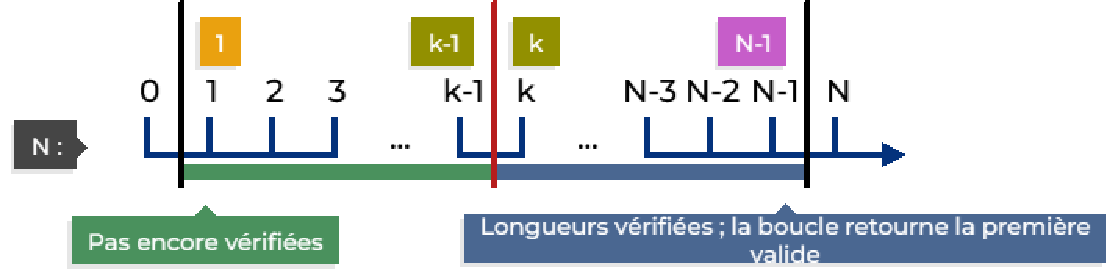
\includegraphics[width=1\textwidth]{invariant-1.pdf}
    \caption{Invariant graphique SP1}
\end{figure}

\subsection{SP2:}
\textbf{Invariant formel:} \\
    $ T = T_0 \land N = N_0 \land k = k_0$ \\
    $\land$ \\
    $0 \leq i < k$ \\
    $\land$ \\
    $T[i] = T[N - k + i]$ \\

\begin{figure}[h]
    \centering
    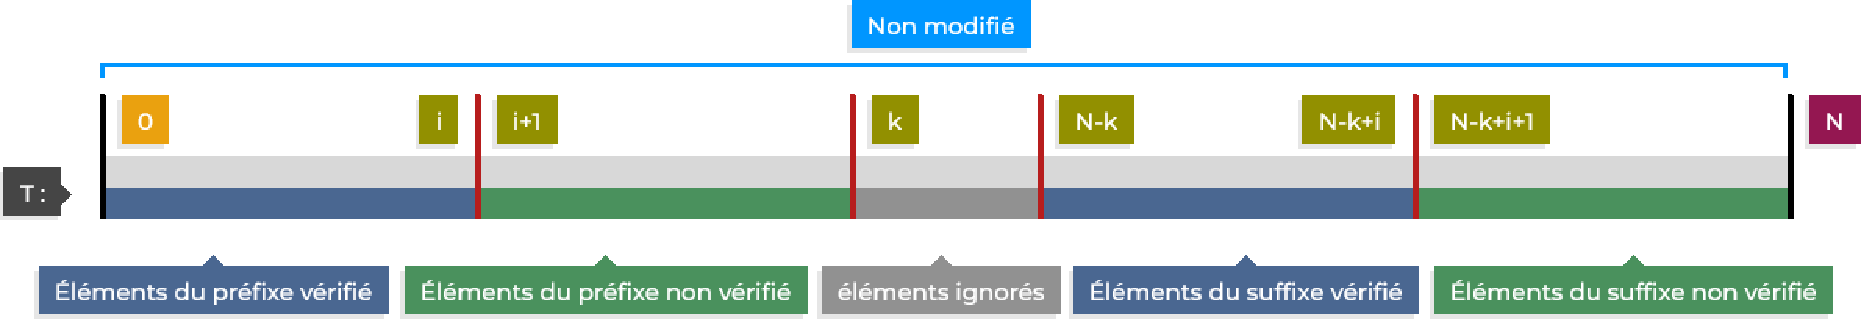
\includegraphics[width=1\textwidth]{invariant-2.pdf}
    \caption{Invariant graphique SP2}
\end{figure}



% !TEX root = ./main.tex
%%%%%%%%%%%%%%%%%%%%%%%%%%%%%%%%%%%%%%%%%%%%%%%%%%%%%%%%%%%%%%%%%%%%%%%%%%%%%%%%%%%%%%%%%%
% Dans cette section, il est demandé d'appliquer l'approche constructive pour la         %
% construction de votre code.                                                            %
%                                                                                        %
% Pour chaque Sous-Problème (une sous-section/SP):                                       %
% - {Pré} INIT {INV}                                                                     %
% - déterminer le Critère d'Arrêt (et donc le Gardien de Boucle)                         %
% - {INV & B} ITER {INV}                                                                 %
% - {INV & !B} END {Post}                                                                %
% - Fonction de Terminaison (pensez à justifier sur base de l'Invariant Graphique)       %
% (une sous-sous-section/tiret)                                                          %
%%%%%%%%%%%%%%%%%%%%%%%%%%%%%%%%%%%%%%%%%%%%%%%%%%%%%%%%%%%%%%%%%%%%%%%%%%%%%%%%%%%%%%%%%%
\section{Approche Constructive}
%%%%%%%%%%%%%%%%%%%%%%%%%%%%%%%%

\begin{lstlisting}[caption={SP1}]
int prefixe_suffixe(int *T, const unsigned int N) {
    unsigned int k = N - 1;
    // {$T = T_0 \land N =N_0 \land k = N - 1$}
    while (k > 0) {
        // {$0 < k < N \land T = T_0 \land N =N_0$}
        if (pref_equal_suff(T, N, k)) return k;

        // {$T[0..k-1] \neq T[N-k..N-1]$}
        k--;
        // {$k = k - 1$}
    }
    // {$k = 0$}
    return 0;
    // {$T = T_0 \land N = N_0$}
}
\end{lstlisting}




\begin{lstlisting}[caption={SP2}]
static int pref_equal_suff(int *T, const unsigned int N, const unsigned int k) {

    unsigned int i = 0;
    // {$T = T_0 \land N =N_0 \land k = k_0$}
    while (i <= k - 1) {
        // {$T = T_0 \land N =N_0 \land k = k_0 \land 0 \leq i < k$}
        if (T[i] != T[N - k + i]) return 0;
        // {$T[i] = T[N - k + i]$}

        i++;
        //{$i = i + 1$}
    }
    //{$i = k$}
    return 1;
    // {$T = T_0 \land N =N_0 \land k = k_0 \land T[0..k-1] = T[N-k..N-1]$}
    }
\end{lstlisting}


% !TEX root = ./main.tex
%%%%%%%%%%%%%%%%%%%%%%%%%%%%%%%%%%%%%%%%%%%%%%%%%%%%%%%%%%%%%%%%%%%%%%%%%%%%%%%%%%%%%%%%%%
% Dans cette section, indiquez le code complet (sans assertions intermédiaires) de votre %
% solution                                                                               %
%%%%%%%%%%%%%%%%%%%%%%%%%%%%%%%%%%%%%%%%%%%%%%%%%%%%%%%%%%%%%%%%%%%%%%%%%%%%%%%%%%%%%%%%%%
\section{Code Complet}\label{code}
%%%%%%%%%%%%%%%%%%%%%%%

\lstinputlisting[caption=Implémentation de prefixe\_suffixe]
    {../code/prefixe_suffixe.c}


% !TEX root = ./main.tex
%%%%%%%%%%%%%%%%%%%%%%%%%%%%%%%%%%%%%%%%%%%%%%%%%%%%%%%%%%%%%%%%%%%%%%%%%%%%%%%%%%%%%%%%%%
% Dans cette section, vous devez étudier complètement la complexité de votre code.       %
% Soyez le plus formel (i.e., mathématique) possible.                                    %
%%%%%%%%%%%%%%%%%%%%%%%%%%%%%%%%%%%%%%%%%%%%%%%%%%%%%%%%%%%%%%%%%%%%%%%%%%%%%%%%%%%%%%%%%%
\section{Complexité}\label{complexite}
%%%%%%%%%%%%%%%%%%%%

\textbf{Complexité de \texttt{pref\_equal\_suff}}:
\begin{itemize}
    \item Complexité exacte:\\
        $ T_1(k) = 1 + (k+1) + k + k + 1 = 3k + 3$\\
    \item Asymptotique:\\
        $ T_1(k) \in \mathcal{O}(k) $
\end{itemize}

\textbf{Complexité de \texttt{prefixe\_suffixe}}:
\begin{itemize}
    \item Complexité exacte:\\
        \[
        T_2(N) = 1 + \sum_{k=N-1}^{1} [3 + T_1(k)] + 1
        = 2 + 3 \sum_{k=N-1}^{1} [3k + 6]
        = 2 + \frac{3(N-1)N}{2} + 6(N - 1)
        = \frac{3N^2 - 3N}{2} + 6N - 4
        \]
    \item Asymptotique:\\
        $ T_2(N) \in \mathcal{O}(N^2) $
\end{itemize}



% !TEX root = ./main.tex
%%%%%%%%%%%%%%%%%%%%%%%%%%%%%%%%%%%%%%%%%%%%%%%%%%%%%%%%%%%%%%%%%%%%%%%%%%%%%%%%%%%%%%%%%%
% Rédigez ici la conclusion de votre rapport.                                            %
%%%%%%%%%%%%%%%%%%%%%%%%%%%%%%%%%%%%%%%%%%%%%%%%%%%%%%%%%%%%%%%%%%%%%%%%%%%%%%%%%%%%%%%%%%
\section{Conclusion}\label{conclusion}
%%%%%%%%%%%%%%%%%%%%%

% C'est un cours difficile

Pour terminer ce rapport nous pouvons ajouter que nous avons réussi à créer un algorithme
en C cappable de trouver le plus long préfixe qui est aussi un suffixe d'une liste donnée.
Et tout cela en respectant les contraintes données tel que l'utilisation exclusives des
boucles while et l'abscence de l'utilisation de list intermédiaires.


%%%%%%%%%%%%%%%%%%%% FIN DE LA ZONE PROTÉGÉE %%%%%%%%%%%%%%%%%%%%

\end{document}
